\chapter{Quality Assurance}
\label{chap:testing_system_evaluation}

This chapter presents the quality assurance activities used to evaluate \gls{SafeVision}. It describes the overall testing strategy, including frontend testing, backend testing, user testing, performance testing, and security evaluation. The purpose of the chapter is to assess both the technical correctness of the system and its practical suitability for detecting, reviewing, and anonymizing sensitive information in visual media.


\section{Testing Strategy}

A layered testing strategy was used to evaluate \gls{SafeVision}. At the lowest level, unit tests were written for utility functions, state management, and isolated processing logic. On top of this, integration oriented tests were used for workflows where several hooks, components, or services had to work together. Finally, user oriented evaluation was performed through manual exploratory testing and structured user tests on realistic image and video scenarios in order to assess both practical usability and hybrid workflow behavior.

This combination was chosen because no single testing method was sufficient on its own. Unit tests gave fast feedback and were useful for regression prevention, while integration tests validated interactions across components and services. Manual and user based testing were necessary for evaluating workflows involving file handling, media rendering, and user-controlled redaction, where visual feedback and interaction design played a central role.

In addition to verifying correctness and usability, the user-oriented evaluation was also used to better understand practical user needs. Feedback from real users and users with experience in image and video editing provided insight into different aspects for the system.

\section{Frontend Testing}

Frontend testing was conducted using Vitest in combination with React Testing Library within a JSDOM-based environment. This setup was well suited to the React and Vite architecture of \gls{SafeVision}, allowing both isolated logic and component-level interactions to be tested in a lightweight and reproducible manner.

The frontend test suite covered functionality central to the \gls{SafeVision} workflow, including file handling, consent management, detection and highlight state, workspace interaction, and media controls. Tests also covered utility functions related to image editing, canvas export, video playback, and manifest handling. Since the system supports both images and video, the test suite included checks for frame based operations and synchronization of state across video interactions. This helped verify that core user workflows remained stable across both image and temporal media processing.

\begin{table}[H]
\centering
\small
\begin{tabular}{lcccc}
\hline
\textbf{Module} & \textbf{Statements} & \textbf{Branches} & \textbf{Functions} & \textbf{Lines} \\
\hline
Overall Coverage      & 47.58\% & 38.22\% & 51.37\% & 49.82\% \\
Application Core      & 65.45\% & 45.83\% & 17.64\% & 70.58\% \\
Detection Features    & 50.70\% & 30.43\% & 52.00\% & 47.16\% \\
File Management       & 60.72\% & 29.05\% & 63.23\% & 62.96\% \\
User Preferences      & 50.98\% & 41.66\% & 36.84\% & 56.81\% \\
Workspace Components  & 66.66\% & 66.66\% & 63.63\% & 64.28\% \\
Workspace Hooks       & 32.02\% & 13.00\% & 52.17\% & 35.06\% \\
Image Processing      & 21.48\% & 4.87\%  & 18.75\% & 22.03\% \\
Video Processing      & 22.72\% & 18.69\% & 19.29\% & 24.65\% \\
Shared UI Hooks       & 71.16\% & 44.96\% & 80.48\% & 75.00\% \\
Storage / Persistence & 41.48\% & 48.03\% & 41.66\% & 44.67\% \\
UI Components         & 41.75\% & 49.03\% & 40.00\% & 40.00\% \\
\hline
\end{tabular}
\caption{Frontend test coverage grouped by major application modules. }
\label{tab:frontend_coverage}
\end{table}
 
In total, the frontend test suite from ~\ref{tab:frontend_coverage} consisted of 38 test files containing 164 passing tests. Coverage was strongest in state management, shared \acrshort{ui} hooks, and utility-driven logic. While lower coverage was observed in larger \acrshort{ui} components and media-heavy modules, particularly within image and video rendering workflows. This is largely due to the complexity of browser \acrshort{api}s, asynchronous rendering behavior, and canvas/video interactions, which are inherently more difficult to test automatically than deterministic application logic. Despite this, core interaction flows involving editing, file management, and state transitions were consistently validated through automated tests.

The distribution of coverage reflects the architectural priorities of the system. Logic heavy modules achieved higher coverage due to their deterministic behavior and ease of isolation, while interactive rendering layers achieved lower coverage because they depend heavily on simulated browser behavior. Although full coverage was neither practical nor necessary within the scope of this project, the implemented test suite provided strong regression protection for the most critical frontend functionality.


\section{Backend Testing}

Backend testing was conducted using pytest together with FastAPI's TestClient and the pytest-cov coverage plugin. This setup made it possible to test both isolated backend logic and full API endpoint behavior in a controlled and reproducible way. The backend test strategy combined unit oriented tests for internal processing logic with integration oriented tests for route handling, request validation, and service level workflows.

Particular emphasis was placed on the parts of the backend most central to system correctness and reliability. This included API controllers, detection and redaction services, core processing pipelines, frame based video processing, runtime configuration, and FFmpeg related startup validation. Endpoint level tests were executed through the FastAPI application using a test client, allowing route registration, validation behavior, error handling, and response formats to be verified without deploying the backend as a running service. Lower level functions and processing modules were tested in isolation, often with mocked dependencies to avoid unnecessary reliance on heavy runtime components.

The backend test suite covered both image based and video based workflows. Detection endpoints, redaction endpoints, and video processing controllers were tested for both valid and invalid inputs. In cases where backend functionality depended on larger processing pipelines or external model calls, mocking was used to isolate controller and service behaviour from the underlying implementation. This made the tests faster, more deterministic, and better suited for regression testing. The same approach was also used for startup and lifecycle testing, where environment dependent operations such as FFmpeg verification were simulated rather than executed directly.

In addition to the automated backend test suite, selected API endpoints were also verified manually using Postman. While local API calls were useful during development and debugging, the final manual verification was primarily performed against the deployed backend in order to confirm correct request handling, multipart file upload behavior, and response structure in a production-like environment. Figure~\ref{fig:postman_detect_backend} shows an example of such manual verification for the deployed detection endpoint.

\begin{figure}[H]
    \centering
    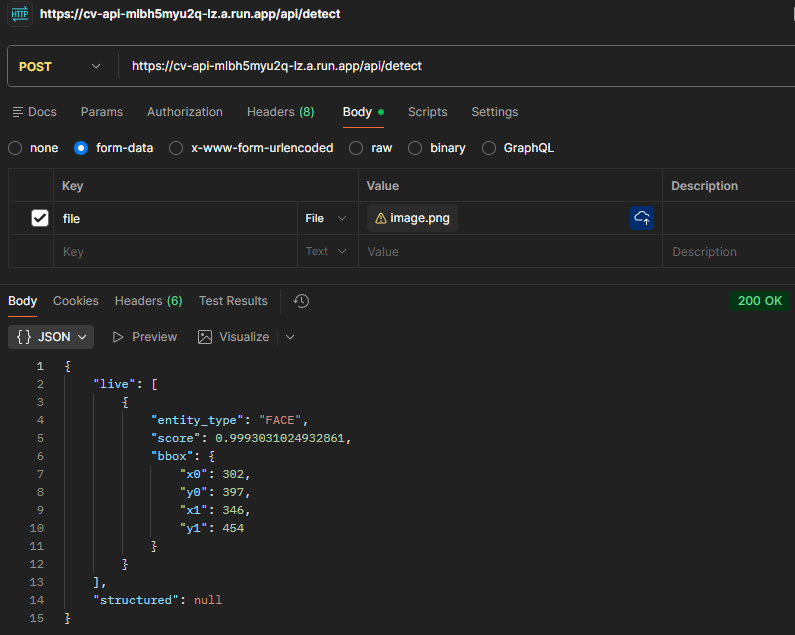
\includegraphics[width=0.80\textwidth]{figures/images/chapter-10/postman_example.png}
    \caption{Manual verification of the deployed \texttt{/api/detect} endpoint in Postman, showing multipart image upload and the returned structured JSON response.}
    \label{fig:postman_detect_backend}
\end{figure}

Coverage analysis showed strong overall backend verification. The backend reached 99\% total statement coverage, with especially high coverage in controllers, startup logic, shared processing modules, and central service layers. Several of the most important files for application behavior, including \texttt{main.py}, the controller modules, \texttt{detector\_service.py}, \texttt{frame\_live.py}, \texttt{video\_live.py}, and \texttt{pipeline\_core.py}, achieved full coverage. This indicates that the most critical backend paths for request handling, orchestration, and media processing were thoroughly exercised by the automated test suite. A complete per-file backend coverage report is provided in Appendix~\ref{appendix:backend_coverage_full}.

\begin{table}[H]
\centering
\small
\begin{tabular}{lc}
\hline
\textbf{Backend Module Group} & \textbf{Coverage} \\
\hline
Overall Backend Coverage & 96\% \\
Application Entry / Startup & 100\% \\
Controllers / API Routes & 100\% \\
Core Pipeline Modules & 100\% \\
Video Processing Core & 100\% \\
Detection Service Layer & 100\% \\
Text Analysis (PII detector) & 94\% \\
Tracking Utilities & 96--99\% \\
\hline
\end{tabular}
\caption{Summary of backend test coverage across key module groups}
\label{tab:backend_coverage}
\end{table}

Although backend coverage was high overall, the few modules with lower individual coverage were still exercised through the surrounding backend architecture. Since these components are invoked by higher level services, pipelines, and API routes, much of their practical behavior was verified indirectly through integration oriented tests. Consequently, lower isolated file coverage in these cases does not mean that the functionality was left untested, but rather that it was validated primarily as part of larger execution flows.

Overall, the backend testing process provided strong confidence in the correctness and robustness of \gls{SafeVision}'s server side functionality. The combination of route level verification, service and pipeline testing, targeted mocking of environment dependent dependencies, and manual \acrshort{api}. Verification made it possible to validate both internal logic and realistic request flows while keeping the test suite efficient and maintainable.

\section{User Testing}
\label{sec:user-testing}

User testing was conducted in multiple phases throughout the development period, with each batch corresponding to a different stage of system maturity and providing progressively more targeted insights. The initial tests, conducted in mid-March, were designed to gather both qualitative feedback on how users perceived and interacted with the system and quantitative data on usability challenges and problematic aspects. These early sessions offered a broad understanding of user behavior and highlighted key areas of difficulty. In subsequent phases, the design and execution of the tests were refined, allowing for more targeted data collection and a clearer evaluation of specific usability issues and system improvements.

\methodheading{UI Changes Based on User Testing}

Based on findings from the initial testing phases and feedback from relevant user groups (Appendix ~\ref{app:user_test_phase_1}), several changes were implemented to improve the usability and clarity of the system. The changes were aimed not only at resolving usability issues, but also at better aligning the system with practical user needs. Feedback from Skan-Kontroll emphasized that the system needed to support efficient processing, clear workflow progression, and reliable manual control over detection results. Feedback from users with image and video editing experience further highlighted the importance of predictable interaction patterns, editing precision, and clear feedback during longer processing tasks.

The most frequently observed usability issues are summarized in Table~\ref{tab:user_test_summary}. The results show that challenges related to detection feedback, workflow understanding, and navigation were among the most common problems experienced by users.

\begin{table}[h]
\centering
\begin{tabular}{lc}
\hline
\textbf{Usability Issue} & \textbf{Out of 10 Users} \\
\hline
Difficulty navigating to detection & 5 \\
Unclear detection/scanning feedback & 7 \\
Confusion about workflow steps & 6 \\
Uncertainty about system state & 4 \\
Difficulty understanding terminology & 3 \\
Issues with redaction process & 4 \\
\hline
\end{tabular}
\caption{Summary of recurring usability issues identified across initial testing phases}
\label{tab:user_test_summary}
\end{table}

In response to these findings, several interface and interaction changes were introduced. One of the main adjustments was a restructuring of the interface flow. The order of key action buttons was modified to better reflect the natural progression of tasks, making it easier for users to understand what to do next. In addition, the feature previously labeled as ``AI mission'' was renamed to ``Identify'' in order to provide clearer and more intuitive terminology, as suggested by Thomas Berg Fjellestad Appendix ~\ref{app:meeting-2026-03-17}.

To improve system feedback, loading indicators were introduced for individual files during processing. This included both the identification step and the redaction process, allowing users to better understand the current state of the system and reducing uncertainty during longer operations.

The April feedback was coded using the same recurring usability categories as the initial testing summary, making it possible to compare whether the main issues became less frequent after the interface and workflow changes. The results are summarized in Table~\ref{tab:user_test_after}. Compared with the initial testing phases, unclear detection feedback and terminology-related problems occurred less frequently, suggesting that the added progress bar and clearer terminology helped reduce some of the earlier uncertainty. However, the results also show that some challenges remained, particularly around workflow understanding and manual redaction.

\begin{table}[H]
\centering
\begin{tabular}{lc}
\hline
\textbf{Usability Issue} & \textbf{Out of 10 Users} \\
\hline
Difficulty navigating to detection & 5 \\
Unclear detection/scanning feedback & 2  \\
Confusion about workflow steps & 6 \\
Uncertainty about system state & 3  \\
Difficulty understanding terminology & 2 \\
Issues with redaction process & 6 \\
\hline
\end{tabular}
\caption{Summary of recurring usability issues identified across the April testing phase after interface and workflow improvements}
\label{tab:user_test_after}
\end{table}

The remaining issues were mainly related to users needing time to understand the first step after uploading media, as well as difficulties with editing overlapping boxes, identifying when manual tools were active, or deleting selected regions. These findings suggest that the main workflow became clearer after the implemented changes, but that progress feedback and manual editing support remained areas for further refinement. The April results therefore show improvement in several of the original problem areas, while also identifying more specific interaction issues that became visible once the basic workflow was easier to complete.


\section{Performance Tests}
\label{sec:performance_tests}

As part of the quality assurance process, performance tests were conducted to evaluate the runtime behavior of the \gls{SafeVision} system. These tests measured the latency of detection and redaction operations across different execution environments and scenario configurations. By comparing local CPU, local \gls{gpu}, and deployed cloud execution, the evaluation provides a practical view of how the system performs under different operational conditions. \Gls{inpainting} was excluded from the performance tests because the evaluation was limited to the redaction methods used most consistently in the core workflow.


\methodheading{Test Setup}

Performance was measured as total API response time per image. The reported latency therefore includes request handling, image upload, backend processing, and response generation. Detection and redaction were measured separately, using the scenario sets summarized in Table~\ref{tab:det_red_scenarios}.

\begin{table}[H]
\centering
\small
\begin{tabularx}{0.8\textwidth}{X X}
\toprule
\textbf{Detection scenarios} & \textbf{Redaction scenarios} \\
\midrule
\texttt{face\_only} & \texttt{blur\_box} \\
\texttt{text\_only} & \texttt{pixelate\_box} \\
\texttt{barcode\_only} & \texttt{blackbox\_box} \\
\texttt{license\_plate\_only} & \texttt{blur\_segmentation} \\
\texttt{object\_only} & \texttt{pixelate\_segmentation} \\
\texttt{all\_enabled} & \texttt{blackbox\_segmentation} \\
\bottomrule
\end{tabularx}


\caption{Detection and redaction scenarios included in the performance tests.}
\label{tab:det_red_scenarios}
\end{table}

For \gls{segmentation} based redaction, only \gls{segmentation} compatible detections were included. In addition, the number of \gls{segmentation} candidates was capped in order to avoid unrepresentative worst-case behavior on densely detected images. The performance measurements were collected across three execution environments, summarized in Table~\ref{tab:performance_environments}.

\begin{table}[H]
\centering
\begin{tabular}{|p{2.6cm}|p{4.3cm}|p{3.2cm}|p{4.2cm}|}
\hline
\textbf{Environment} & \textbf{Hardware / Runtime} & \textbf{Memory} & \textbf{Characteristics} \\ \hline

\textbf{Local CPU} & 
AMD Ryzen 7 5800X3D (8 cores, 16 threads) & 
32 GB RAM & 
CPU-only local execution used as the baseline environment. \\ \hline

\textbf{Local GPU} & 
NVIDIA GeForce RTX 4080 & 
16 GB dedicated \gls{gpu} memory & 
Local \gls{gpu}-accelerated execution for PyTorch-based detectors. \acrshort{ocr} remained CPU-based. \\ \hline

\textbf{Cloud} & 
Google Cloud Run (2 vCPU) & 
8 GiB memory & 
Deployed CPU-based \acrshort{api} environment with concurrency set to 1 and a minimum of 1 instance. \\ \hline

\end{tabular}
\caption{Execution environments used in the performance tests.}
\label{tab:performance_environments}
\end{table}


\methodheading{Detection Performance}

Figure~\ref{fig:detect_latency_by_environment} shows the mean detection latency across the three environments. The local \gls{gpu} environment achieved the lowest latency overall for the most computationally demanding scenarios, particularly for \texttt{face\_only} and \texttt{all\_enabled}. This indicates that the PyTorch-based detection pipelines benefited substantially from \gls{gpu} acceleration.

\begin{figure}[H]
    \centering
    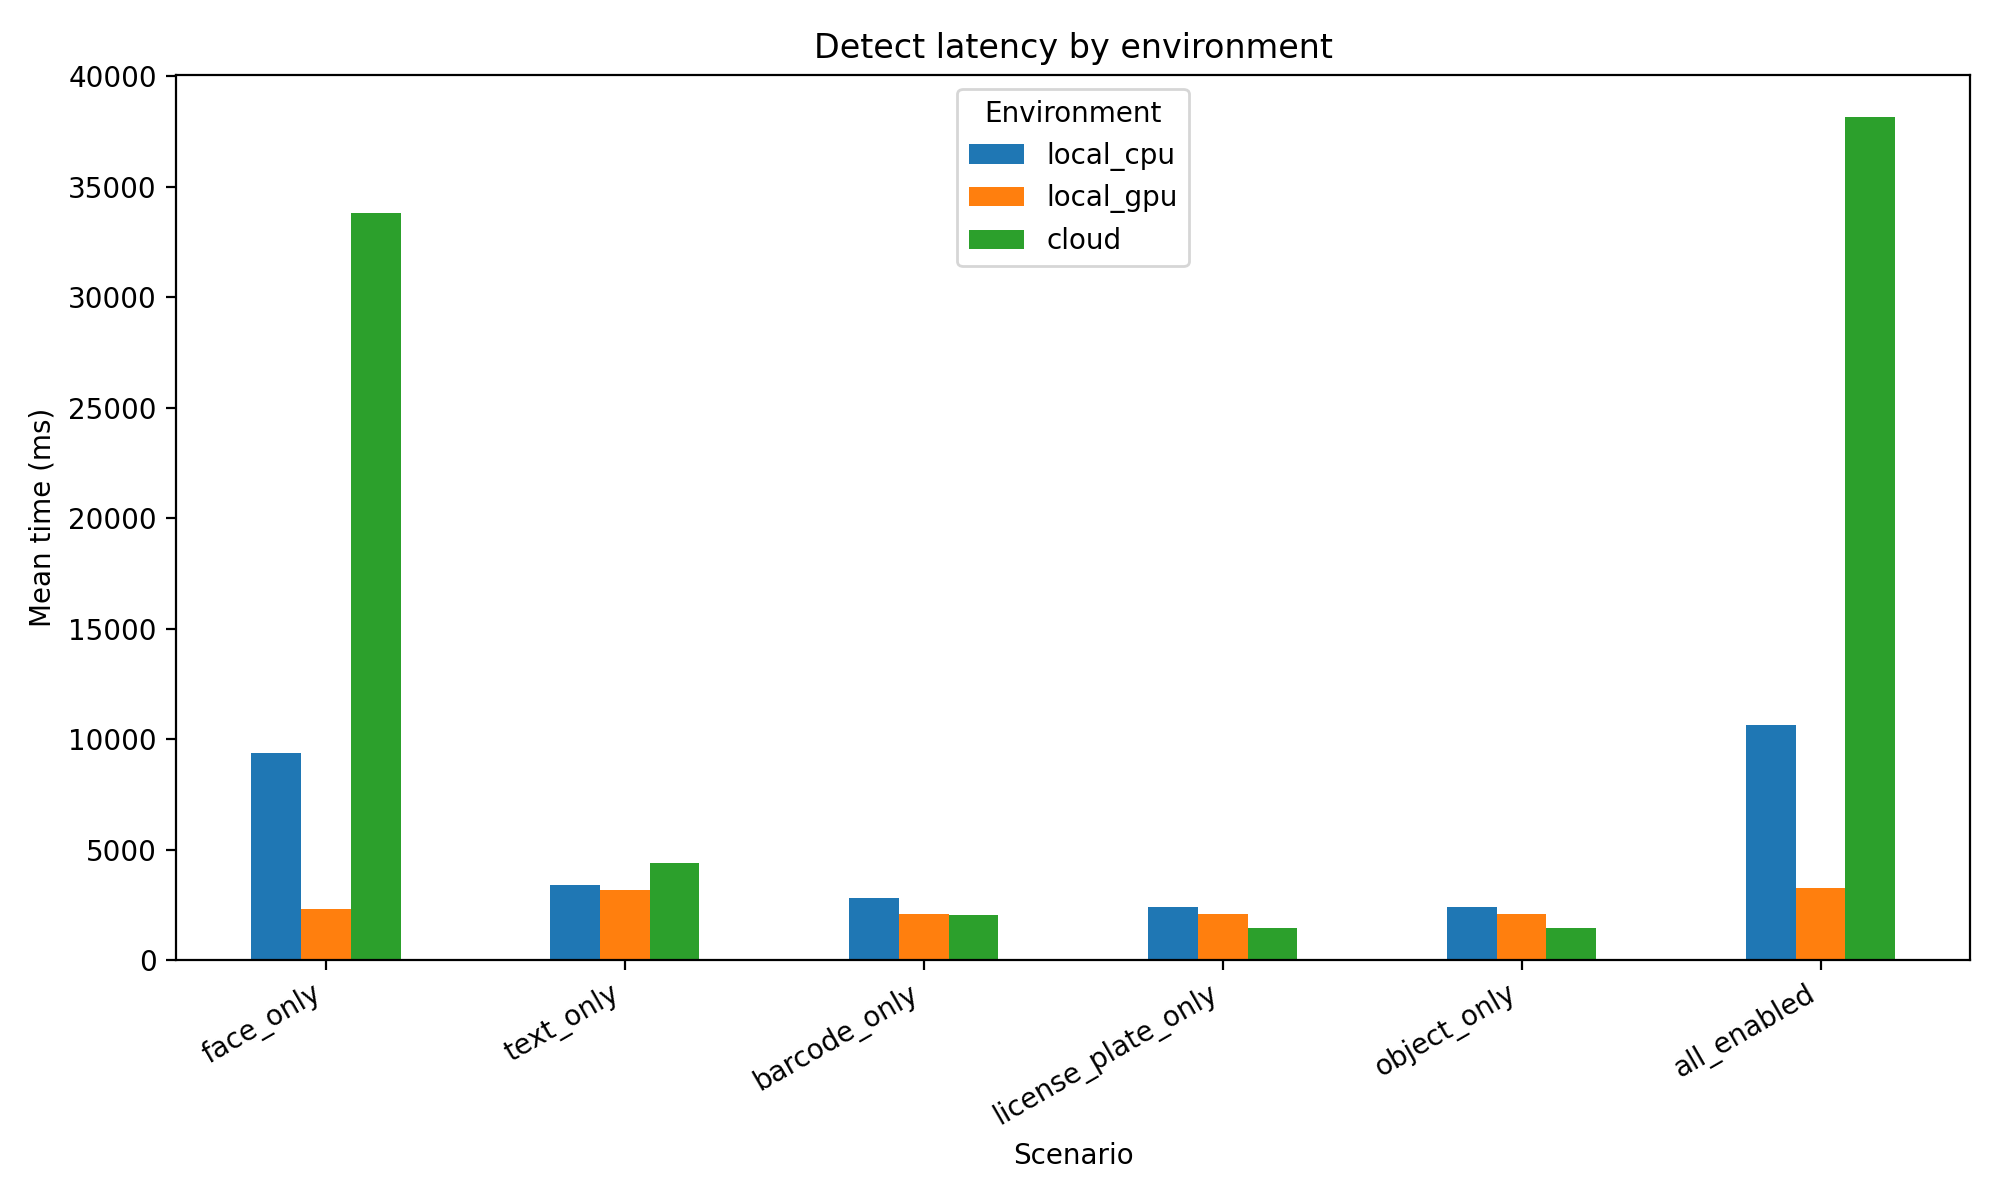
\includegraphics[width=1.1\textwidth]{figures/images/chapter-9/detect_latency_by_environment.png}
    \caption{Mean detection latency across local CPU, local \gls{gpu}, and cloud environments.}
    \label{fig:detect_latency_by_environment}
\end{figure}

The results do not, however, show a uniform ranking across all scenarios. For lighter detection tasks such as \texttt{barcode\_only},
\texttt{license\_plate\_only}, and \texttt{object\_only}, the deployed cloud environment produced lower mean latency than the local CPU environment, and in some cases also lower latency than the local \gls{gpu} environment. Since the measurements represent end-to-end \acrshort{api} response time rather than isolated model \gls{inference} time, these differences are likely influenced by a combination of runtime overhead, workload characteristics, and environment-specific execution conditions rather than hardware category alone.

For the more computationally demanding scenarios, the cloud environment showed substantially higher latency than both local environments, especially for \texttt{face\_only} and \texttt{all\_enabled}. For \texttt{text\_only}, the difference between local CPU and local \gls{gpu} was smaller, which is consistent with the \acrshort{ocr} component remaining CPU-based in the tested local \gls{gpu} configuration. \\


\methodheading{Redaction Performance}

Figure~\ref{fig:redact_latency_by_environment} shows the mean redaction latency across the three environments. For the box-based methods
(\texttt{blur\_box}, \texttt{pixelate\_box}, and \texttt{blackbox\_box}), the results were relatively similar between the local CPU and local \gls{gpu}
environments. This indicates that the redaction stage itself benefited less from \gls{gpu} acceleration than the detection stage. In these scenarios, the cloud environment produced lower mean latency than both local environments.

\begin{figure}[htbp]
    \centering
    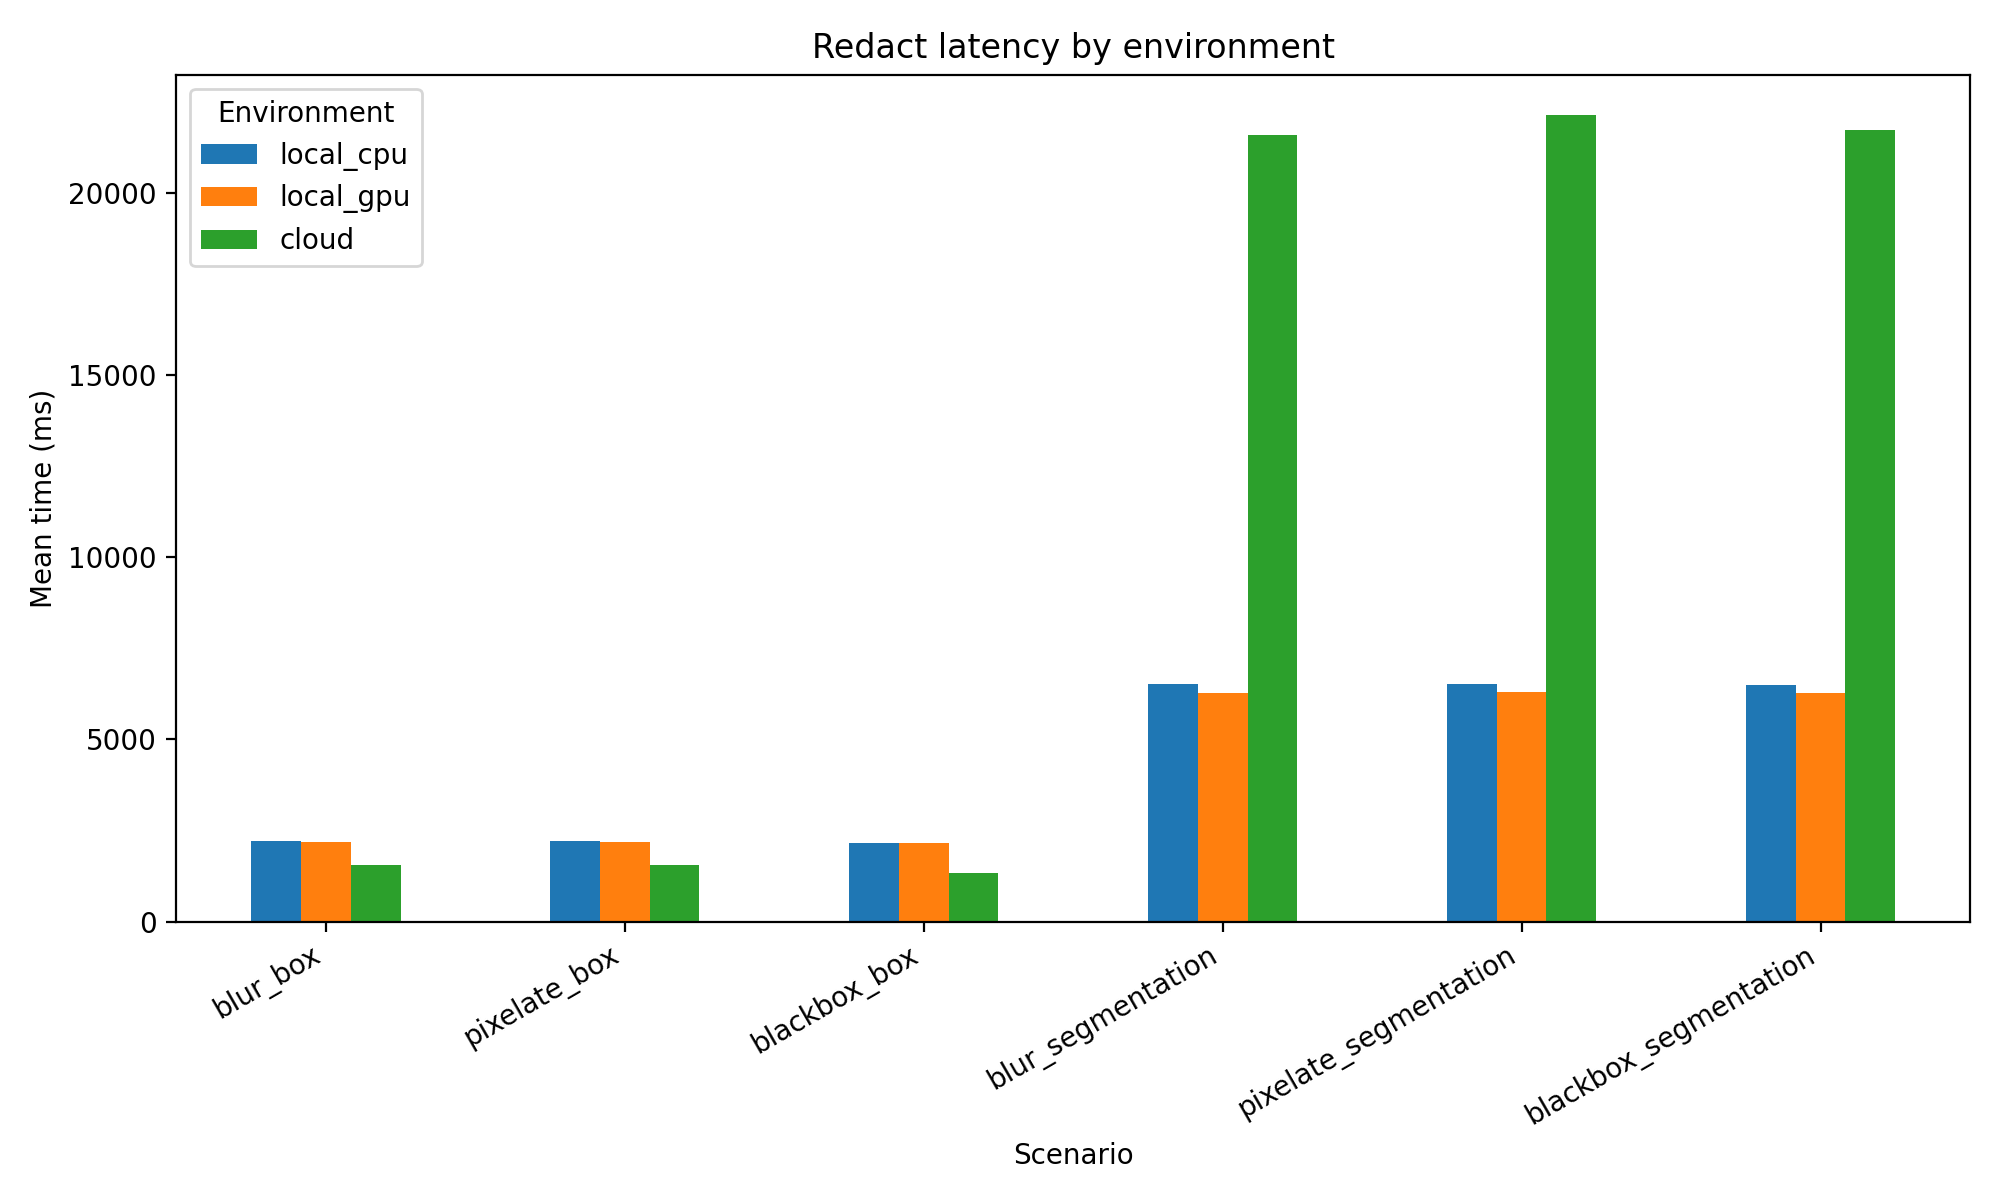
\includegraphics[width=\textwidth,height=0.38\textheight,keepaspectratio]{figures/images/chapter-9/redact_latency_by_environment.png}
    \caption{Mean redaction latency across local CPU, local \gls{gpu}, and cloud environments.}
    \label{fig:redact_latency_by_environment}
\end{figure}

For the \gls{segmentation} based methods (\texttt{blur\_segmentation}, \texttt{pixelate\_segmentation}, and \texttt{blackbox\_segmentation}), the pattern was different. In all three \gls{segmentation} scenarios, the cloud environment showed substantially higher latency than both local environments, while the local CPU and local \gls{gpu} results remained relatively close. This indicates that \gls{segmentation} based redaction introduced a much higher computational cost than box-based redaction, particularly in the deployed cloud setting.

\begin{figure}[htbp]
    \centering
    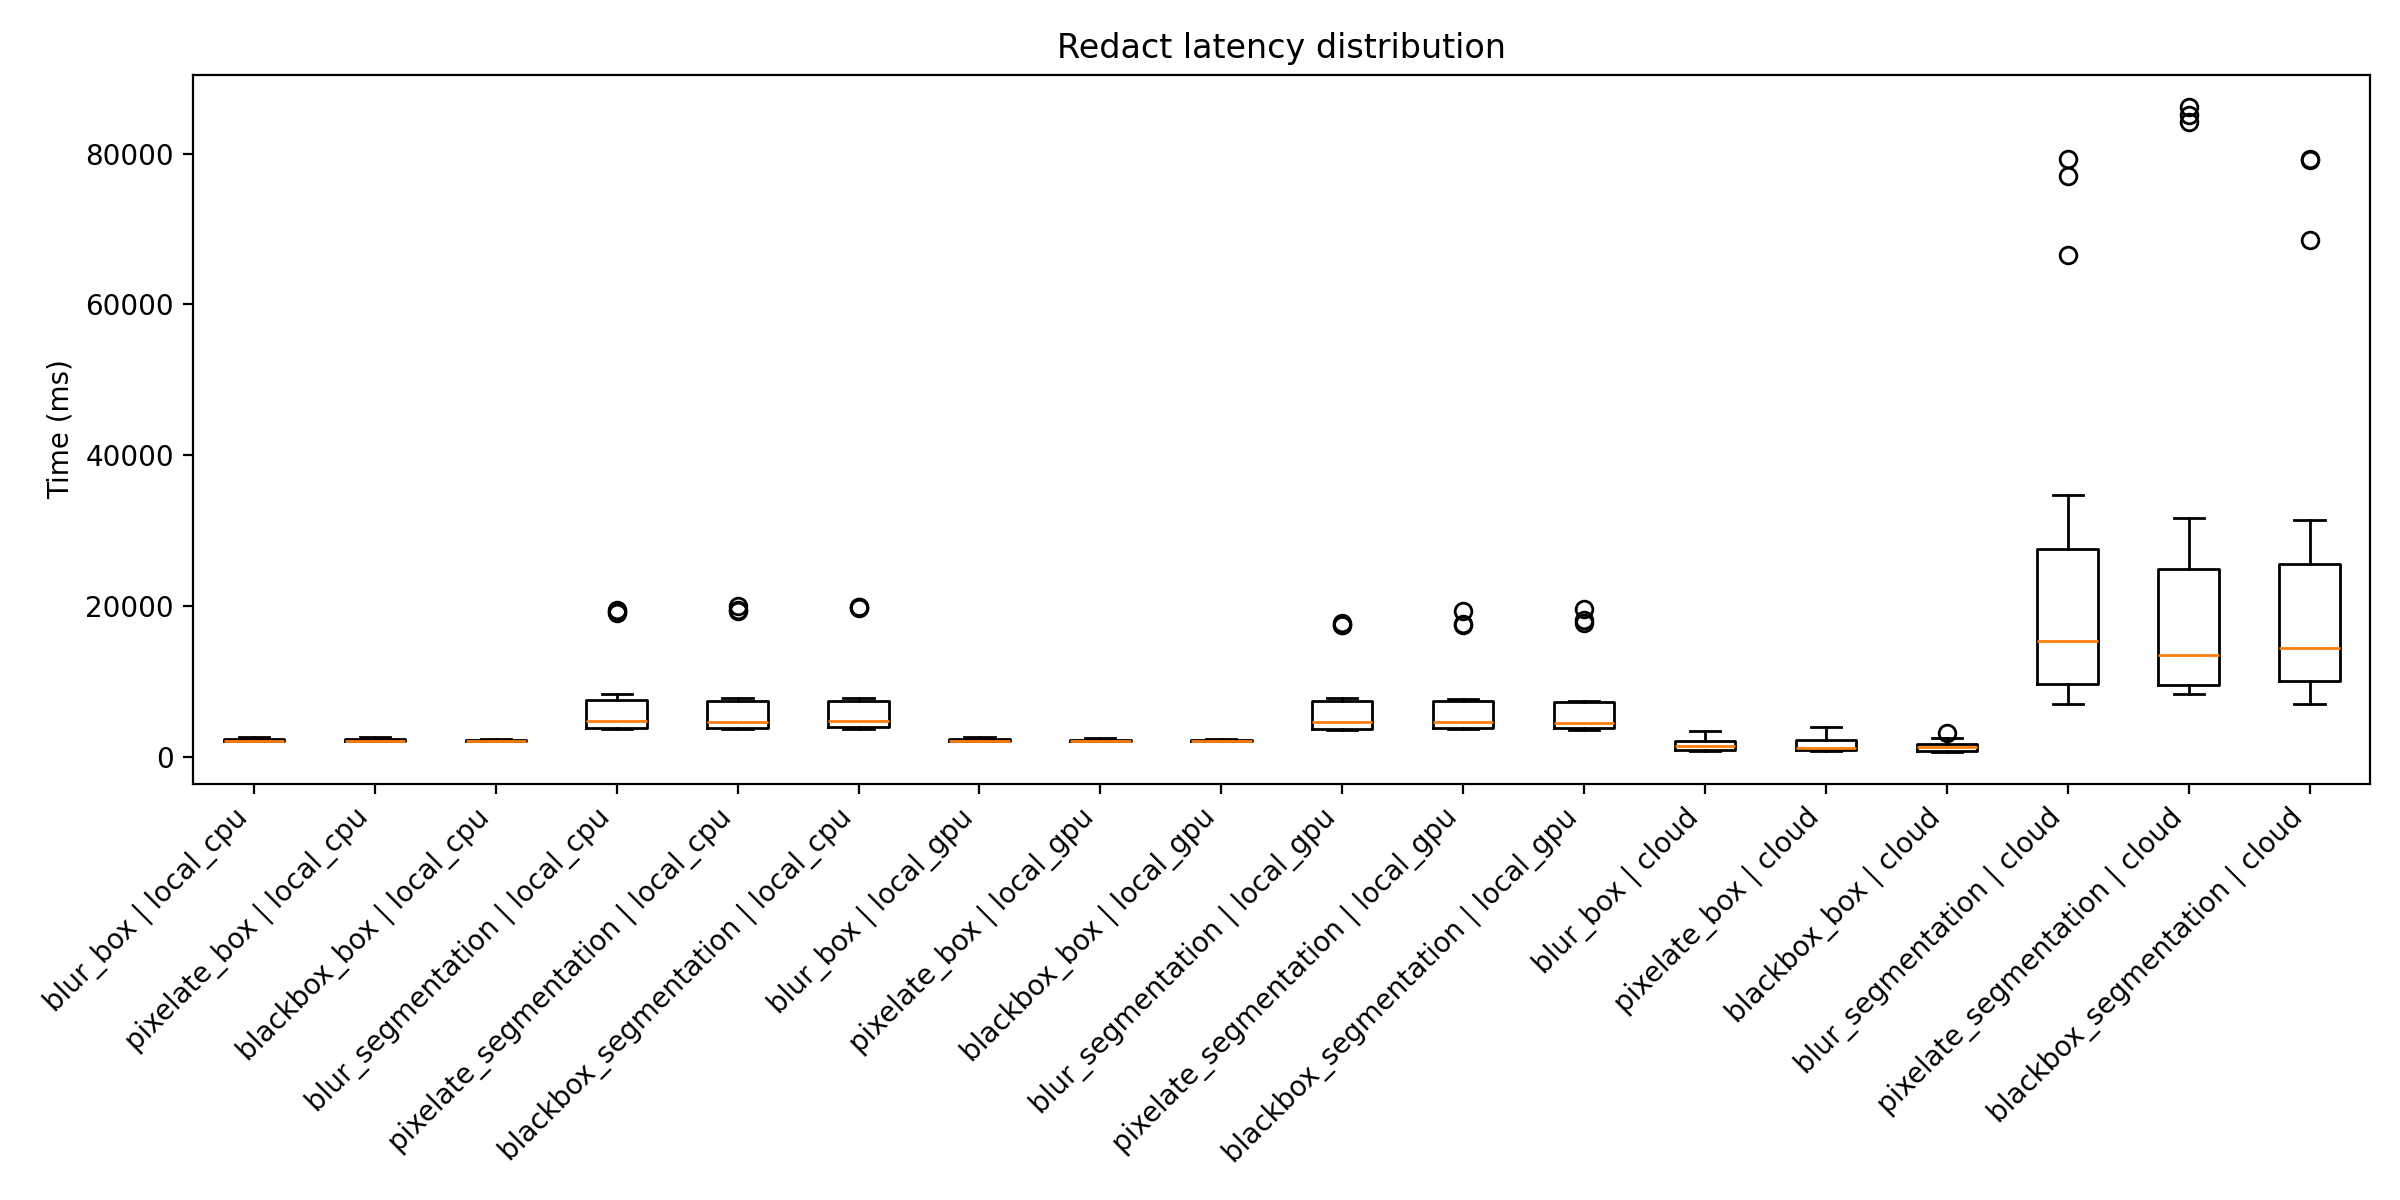
\includegraphics[width=\textwidth,height=0.40\textheight,keepaspectratio]{figures/images/chapter-9/redact_latency_distribution.png}
    \caption{Distribution of redaction latency across scenarios and environments. Lower boxes indicate faster processing, while taller boxes and longer whiskers indicate greater variation between runs. Individual points represent outliers. The cloud \gls{segmentation} scenarios show the highest latency and largest spread.}
    \label{fig:redact_latency_distribution}
\end{figure}

The difference between box-based and \gls{segmentation} based redaction is further illustrated in Figure~\ref{fig:redact_latency_distribution}, which shows that the \gls{segmentation} scenarios had both higher latency and greater variation than the box-based scenarios. This was especially visible in the cloud environment, where \gls{segmentation} based redaction produced the largest spread and the highest outlier values.

Although \gls{segmentation} based redaction was significantly slower, the average number of \gls{segmentation} compatible regions remained low and consistent across environments. This suggests that the increased latency was primarily caused by the \gls{segmentation} process itself rather than by a large number of processed regions. \\

\noindent\textbf{Discussion of Performance Results}

The results show that \gls{gpu} acceleration had the greatest effect on
detection performance, especially for the PyTorch-based detection pipelines. The effect was smaller for text detection, since \acrshort{ocr} remained CPU-based in the tested local \gls{gpu} setup. For redaction, the main distinction was not between \gls{cpu} and \gls{gpu}, but between box-based and \gls{segmentation} based methods. \Gls{segmentation} introduced a significantly higher processing cost in all environments.

The cloud-based measurements were consistently higher for the most demanding scenarios. These results should be interpreted in light of the cloud runtime configuration and the fact that the tests measured end-to-end \acrshort{api} response time rather than isolated model \gls{inference} time. The reported values therefore reflect both processing cost and deployment-related overhead.

\section{Security Evaluation}
\label{sec:security_evaluation}

The security evaluation of \gls{SafeVision} was limited to the attack surface that is relevant for the implemented prototype. The system does not include user authentication, account management, or persistent user databases, and therefore does not expose security concerns such as login bypass, session abuse, or leakage of stored user records. As a result, the evaluation addressed the parts of the system that could be tested meaningfully: \acrshort{api} robustness, malformed input handling, browser-visible data exposure, cross-origin behavior, and client-side storage practices.

The tests documented in Appendix~\ref{app:pen_test} therefore represent the most relevant practical penetration oriented evaluation for the current web application. Tests 1--15 of 19 mainly examined whether the backend handled input validation and error handling in a controlled and stable way across both valid and invalid requests. Taken together, these tests indicate that the backend generally rejects malformed or unsupported input through controlled client-side error responses rather than crashes or unstable behavior. 

Among all the penetration test, some findings are particularly important from a broader privacy and security perspective. Test 16 (Appendix~\ref{appsec:pen_test_16}.16) showed that query tampering on the \texttt{/api/detect} endpoint was handled through controlled validation errors. This suggests that the backend does not simply trust client-supplied parameters.

The browser facing findings are especially relevant in light of the privacy-by-design considerations discussed earlier in Chapter~\ref{chap:theoretical_foundation}. Visual media may contain both direct and indirect identifiers, and GDPR-related design constraints require minimizing unnecessary exposure and processing of personal data. In this context, Test 17 (Appendix~\ref{appsec:pen_test_17}.17) showed that uploaded image content was transmitted as binary form-data in the request body rather than exposed in request URLs. Operational settings such as detection parameters appeared in query strings, but the sensitive image content itself was not exposed there.

Test 18 (Appendix~\ref{appsec:pen_test_18}.18) further supports this overall picture. Normal browser use did not reveal unexpected \acrshort{cors} failures, and the backend implementation shown in Listing~\ref{lst:fastapi_routing} uses an explicit \texttt{ALLOWED\_ORIGINS} list rather than a wildcard '\texttt{*}'. Together, these observations suggest that cross-origin access is intended to be limited to expected frontend origins.

Another important result is given by Test 19 (Appendix~\ref{appsec:pen_test_19}.19), which examined client-side storage. As described earlier in Chapter~\ref{chap:technologies_and_methodologies}, \gls{SafeVision} uses browser-side storage mechanisms to support usability and reduce unnecessary server-side persistence. The inspection showed mainly user preferences and workflow related state, which is a positive finding from a privacy perspective, although locally stored data may still remain accessible on the client device. A summary of the most relevant findings is shown in Table~\ref{tab:security_summary}.

\begin{table}[H]
\centering
\small
\begin{tabularx}{\textwidth}{|p{1.5cm}|p{4.4cm}|X|}
\hline
\textbf{Test} & \textbf{Area} & \textbf{Key finding} \\ \hline

\textbf{16} & 
Input validation & 
Query tampering attempts were rejected safely through controlled validation errors. \\ \hline

\textbf{17} & 
Network exposure & 
Sensitive image content was not exposed in request URLs. \\ \hline

\textbf{18} & 
CORS & 
Cross-origin behavior appeared restricted to expected frontend origins. \\ \hline

\textbf{19} & 
Client-side storage & 
Stored browser data mainly consisted of preferences and workflow-related state. \\ \hline

\end{tabularx}
\caption{Key findings from the security evaluation.}
\label{tab:security_summary}
\end{table}

These findings suggest that \gls{SafeVision} follows a practical privacy conscious design. The system handles malformed \acrshort{api} input in a controlled way, does not appear to expose sensitive visual content unnecessarily in URLs, and relies on browser-side storage rather than avoidable server-side persistence. Within its current scope, the system therefore appears reasonably robust and privacy aware.






\section{Irreversibility Verification of Exported Redactions}
\label{sec:irreversibility-verification}

A central security property of \gls{SafeVision} is that exported redacted images must not retain the original pixel content within the redacted region. This section evaluates whether the black box redaction method satisfies this requirement at the pixel level, that is, whether the export process performs a destructive overwrite of the selected region rather than a visual overlay. Although black box redaction is used as the representative example, the underlying principle applies to all redaction methods supported by the system. The mathematical basis for the irreversibility argument and the complete verification script are provided in Appendix~\ref{app:redaction_irreversibility}.

\methodheading{Verification Approach}

A redaction method is privacy preserving in the exported file only if the original pixel values within the redacted region are no longer recoverable from that file alone. To verify this for \gls{SafeVision}, the analysis examined whether the downloaded 
image retained the original pixel data inside the detected region or whether those values had been replaced during export. The evaluation was performed on an image processed through the full \gls{SafeVision} pipeline, including detection, user confirmation, and export.

As \gls{SafeVision} resizes images during export, the coordinate space changes between the original and exported image. The detected region coordinates returned by the backend were therefore scaled to match the exported image before the pixel-level analysis was applied. The original image had a resolution of $4928 \times 3008$ pixels, and the exported redacted image had a resolution of $1400 \times 855$ pixels. The scale factors in the horizontal and vertical directions were 0.2841 and 0.2842, respectively, indicating near-uniform scaling. The original detection region was:
\[
R_{\text{original}} = (823,\; 499,\; 2562,\; 2950),
\]
which, after scaling to the exported image resolution, became:
\[
R_{\text{exported}} = (234,\; 142,\; 728,\; 839),
\]
corresponding to a region of $494 \times 697$ pixels, totalling 344,318 pixels.

The verification evaluated two properties over this region. First, it measured the proportion of pixels in the exported region that were black or near-black, using a tolerance of 15 intensity levels to account for minor differences introduced by down scaling, anti-aliasing, or encoding. Second, it measured the proportion of pixels that differed from the corresponding region in the original image. A threshold of 99\% was applied to both properties, reflecting the 
expectation that a small number of boundary pixels may be affected by scaling artifacts without compromising the integrity of the redaction.

\methodheading{Visual Verification and Results}

Figure~\ref{fig:org_vs_redaction} illustrates the effect of black box redaction on the exported image. The detected region $R$ is outlined prior to redaction and shown replaced by black pixels in the exported file, providing visual confirmation that the content within the region is no longer present. This is further supported by the pixel-level results summarized in Table~\ref{tab:redaction-irreversibility-results}.

\begin{figure}[H]
\centering
\begin{subfigure}{0.48\textwidth}
    \centering
    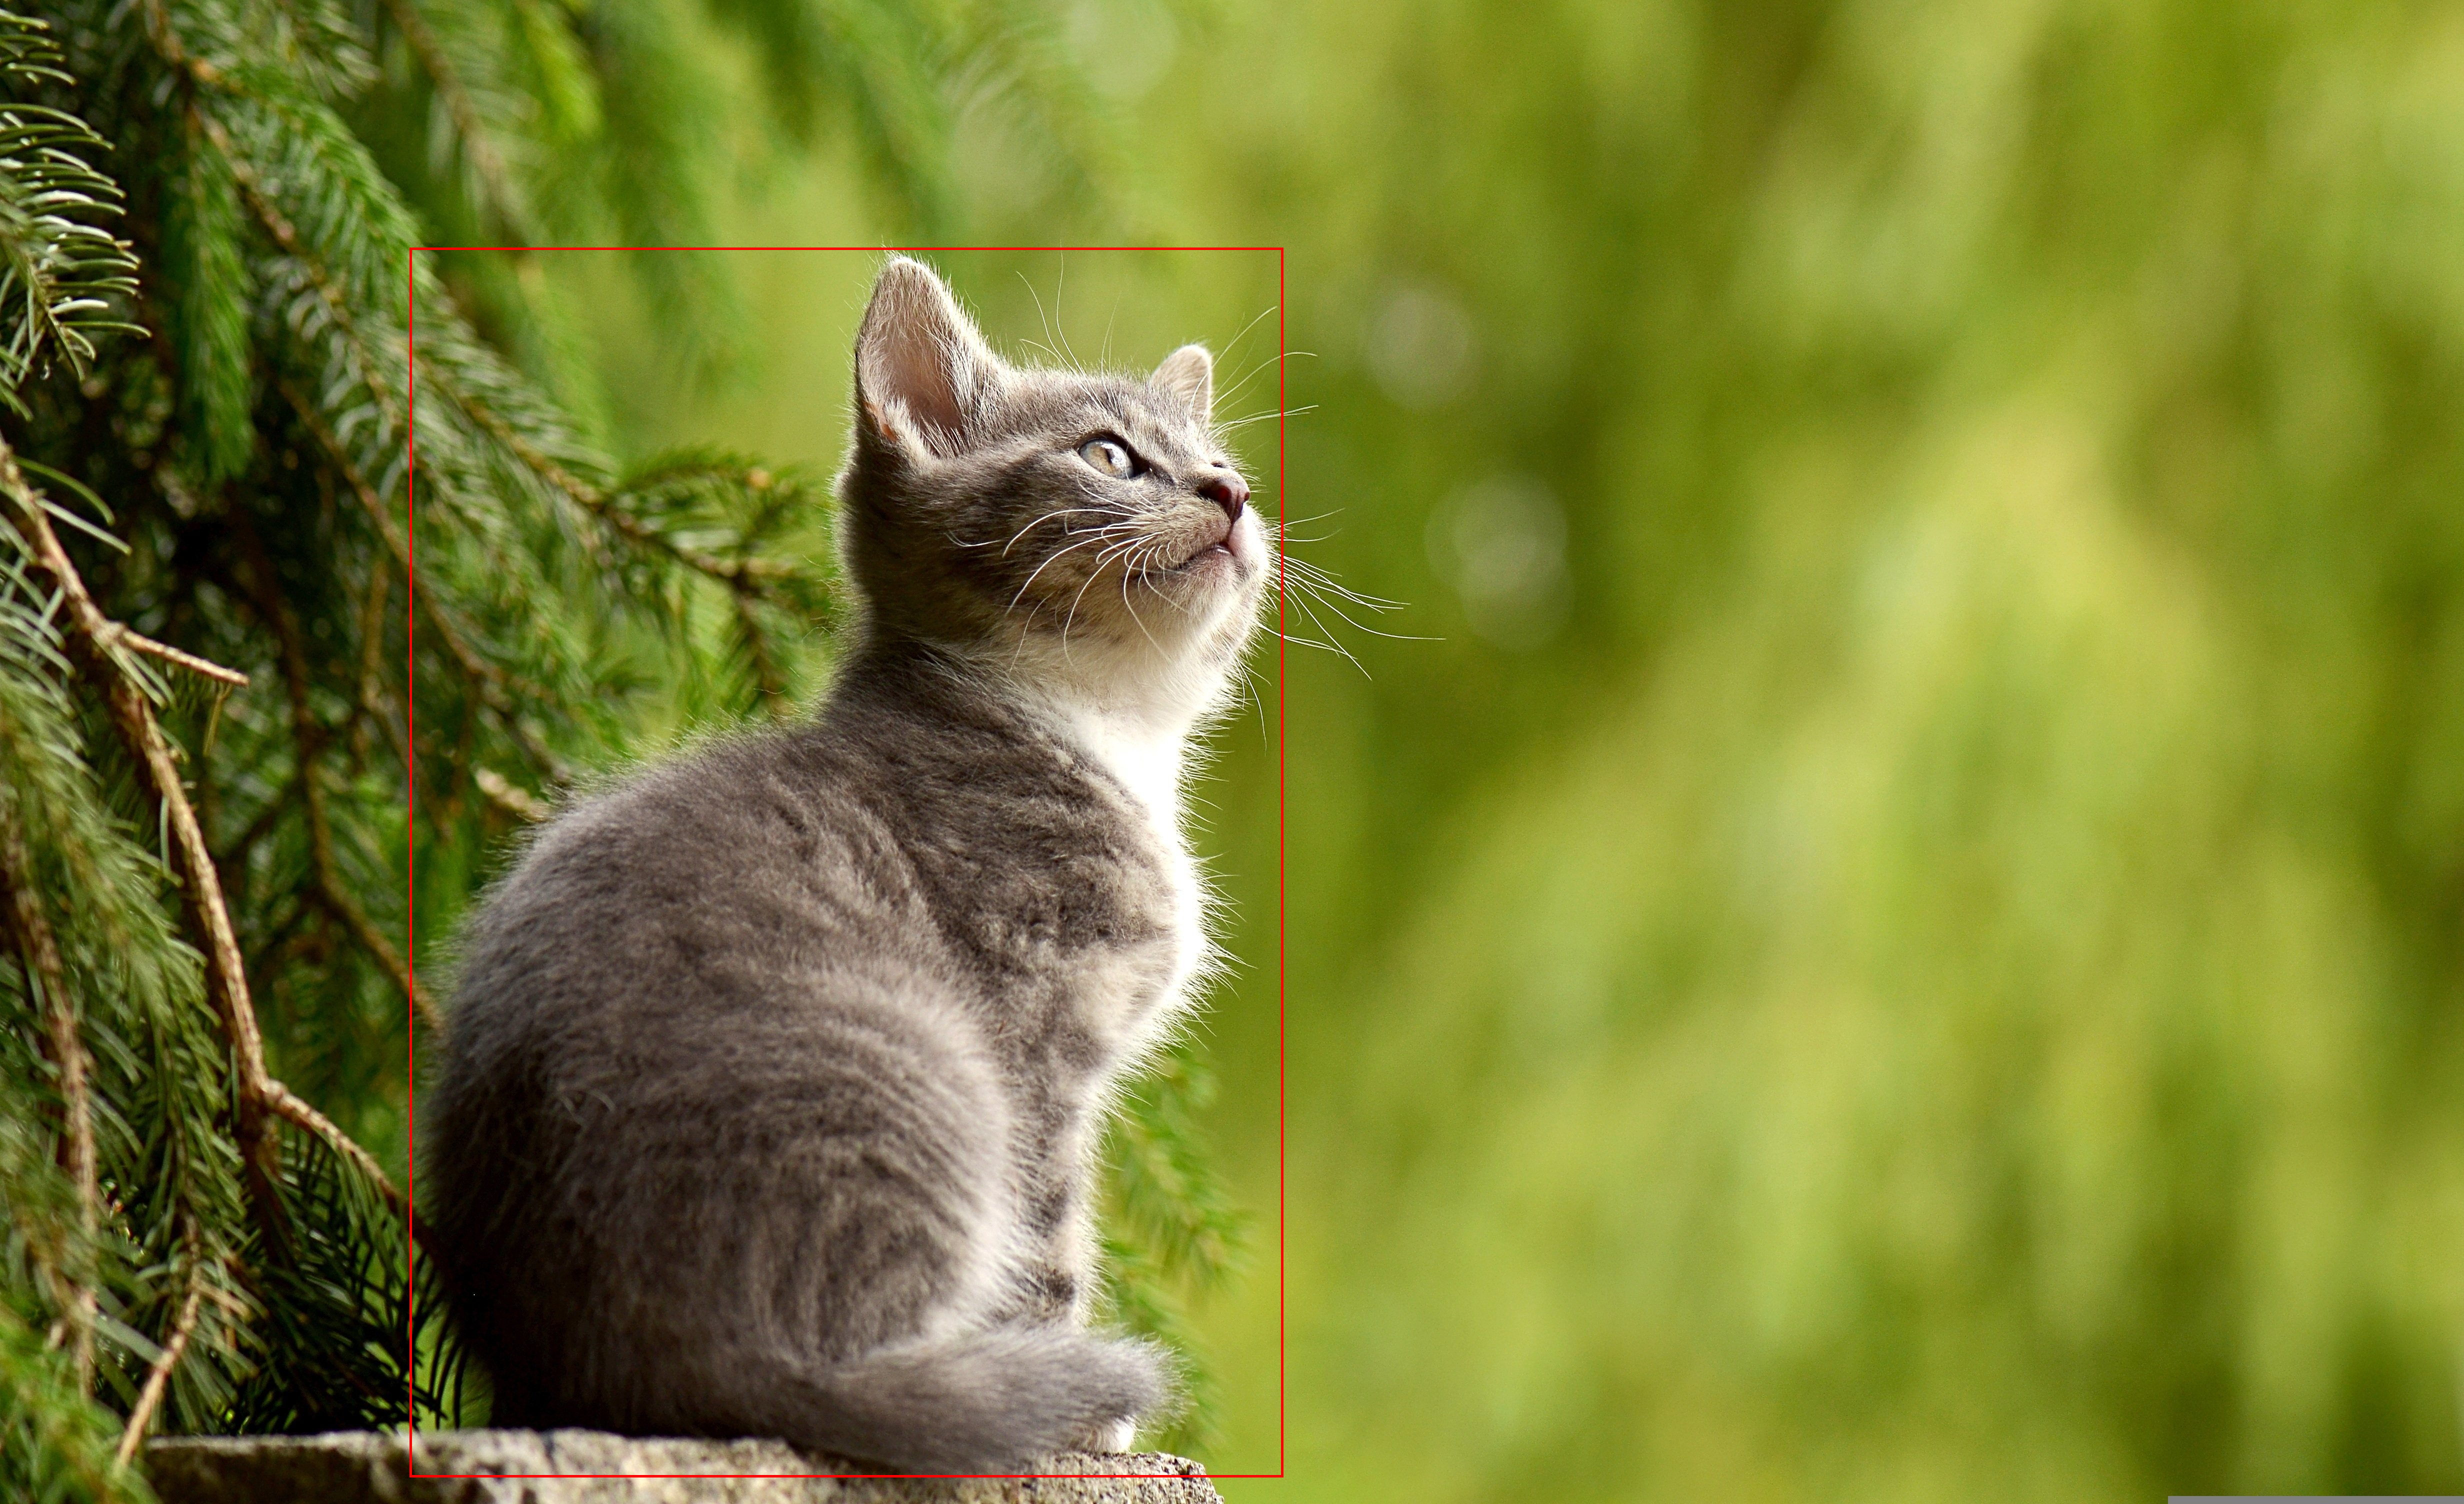
\includegraphics[width=\textwidth]{figures/images/chapter-9/figure_1_original_with_region.png}
    \caption{Original image with the detected region $R$ marked prior to redaction.}
\end{subfigure}
\hfill
\begin{subfigure}{0.48\textwidth}
    \centering
    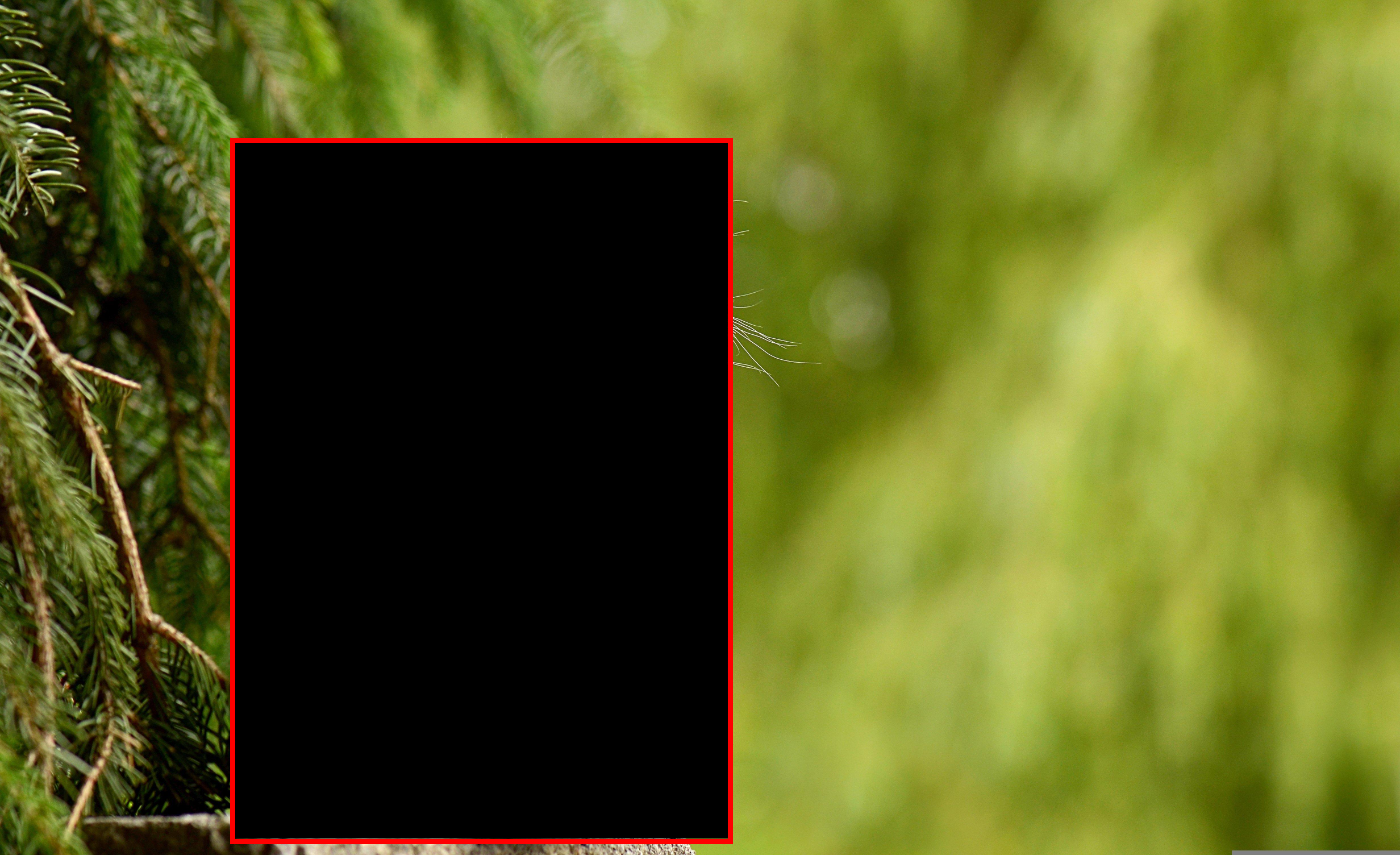
\includegraphics[width=\textwidth]{figures/images/chapter-9/figure_2_redacted_with_region.png}
    \caption{Exported image after redaction, with $R$ scaled to the exported resolution.}
\end{subfigure}
\caption{Comparison of the original and exported redacted image, showing that the 
content within $R$ has been replaced by black pixels. Image source: 
\cite{pixabay_cat_2083492}.}
\label{fig:org_vs_redaction}
\end{figure}

\begin{table}[H]
\centering
\caption{Pixel-level verification results for exported black box redaction.}
\label{tab:redaction-irreversibility-results}
\begin{tabular}{l r}
\toprule
\textbf{Metric} & \textbf{Result} \\
\midrule
Original image size                    & $4928 \times 3008$ \\
Exported image size                    & $1400 \times 855$ \\
Scale factor in x-direction            & 0.2841 \\
Scale factor in y-direction            & 0.2842 \\
Original region coordinates            & $(823,\; 499,\; 2562,\; 2950)$ \\
Scaled exported region coordinates     & $(234,\; 142,\; 728,\; 839)$ \\
Analysed region size                   & $494 \times 697$ pixels \\
Total analysed pixels                  & 344,318 \\
Black or near-black pixels             & 99.857\% \\
Changed pixels compared with original & 99.945\% \\
Metadata in exported PNG               & No EXIF data found \\
Test result                            & Passed \\
\bottomrule
\end{tabular}
\end{table}

Of the 344,318 pixels in the analysed region, 99.857\% were black or near-black within the defined tolerance, and 99.945\% differed from the corresponding pixels in the original image, both exceeding the 99\% threshold. The small proportion of pixels that did not satisfy both criteria is consistent with boundary effects at the edge of the redacted region, where downscaling and anti-aliasing can produce intermediate values. The exported PNG contained no EXIF metadata, indicating that image metadata was not retained during export.

\methodheading{Interpretation and Limitations}

The results confirm that black box redaction in \gls{SafeVision} is destructive at the pixel level in the exported image. The redacted region is not rendered as a visual overlay within the \acrshort{ui} but is instead exported as overwritten pixel data, such that an adversary with access only to the downloaded file cannot recover 
the original content from it. Among the redaction methods supported by the system, black box and solid fill provide the strongest irreversibility guarantees, since they replace original pixel values with a constant. Methods such as blur and pixelation are lossy transformations that derive their output from the original pixels and may preserve partial visual information; these should accordingly be considered weaker from a privacy perspective.

This conclusion is subject to the conditions under which the evaluation was conducted. It applies specifically to the exported redacted file and assumes that an adversary does not have access to the original uploaded image, server-side copies, browser cache, backups, or other external sources that may retain the original data. It is also important to note that irreversibility is a
property of the export process rather than of detection or \gls{segmentation}: those components identify the region $R$, but it is the destructive pixel overwrite during export that establishes the security guarantee evaluated here.






\afterpage{\blankpage}

